\documentclass[spanish, a4paper]{article}

\usepackage{ulem}
\hoffset=-2cm \voffset=-2.5cm
\parskip=0.5cm
\topmargin 2cm

\textwidth 16cm
\textheight 24cm

\usepackage{caratula}
\usepackage[spanish]{babel}
\usepackage[utf8]{inputenc}
%\usepackage[latin1]{inputenc}
\usepackage{fancyhdr} %header lindo
\usepackage{listingsutf8}
\usepackage{pdfpages} %incluir pdf


\usepackage{caption}
\usepackage{subcaption}

\providecommand{\keywords}[1]{\textbf{\textit{Palabras Clave ---}} \textit{#1}}

\usepackage{color}

\definecolor{dkgreen}{rgb}{0,0.6,0}
\definecolor{gray}{rgb}{0.5,0.5,0.5}
\definecolor{mauve}{rgb}{0.58,0,0.82}

\lstset{inputencoding=utf8/latin1}
\lstset{
  frame=none,
  xleftmargin=0.1in,
  stepnumber=1,
  numbers=left,
%  numbersep=5pt,
  numberstyle=\ttfamily\tiny\color[gray]{0.3},
  belowcaptionskip=\bigskipamount,
  captionpos=b,
  escapeinside={*'}{'*},
%  language=Prolog,
  tabsize=1,
%  emphstyle={\bf},
%  commentstyle=\it,
%  stringstyle=\mdseries\rmfamily,
  showspaces=false,
  breaklines=true,
%  keywordstyle=\bfseries\rmfamily,
%  columns=flexible,
%  basicstyle=\small\scriptsize,
  showstringspaces=false,
  morecomment=[l]\%,
}


\pagestyle{fancy}
\lhead{Teoría de Lenguajes}
\rhead{1C 2017}

\newcommand{\persona}[1]{\underline{#1}}

\begin{document}

\fecha{\today}
\titulo{Analizador Sintáctico y Semántico para $\lambda^{bn}$}
\materia{Teoría de Lenguajes}
%\submateria{asd}

\integrante{Gabriel Eric Thibeault}{114/13}{gabriel.eric.thibeault@gmail.com}
\integrante{Gonzalo Ciruelos Rodríguez}{063/14}{Gonzalo.ciruelos@gmail.com}
\integrante{Luis Agustín Nieto}{46/01}{lnieto@dc.uba.ar}

\maketitle

%\tableofcontents

\newpage
\section{Introducción}
En el presente trabajo práctico se realiza un analizador sintáctico y semántico para un subconjunto del cálculo lambda tipado sobre booleanos y naturales $\lambda^{bn}$, para dicha implementación se utilizó PLY que es una implementación en Python de las clásicas herramientas \textit{lex} y \textit{yacc}.

El lexer está implementado en \textit{lexer.py}, en el mismo definimos las expresiones regulares y tokens que sirven para definir si cadenas de entrada son o no válidas acorde a la gramática creada. El parser,donde definimos las producciones de nuestra gramática, está implementado en \textit{parser.py}.\\
Se realizaron una serie de test para probar la correcta implementacion del analizador, los mismos se encuentran en \textit{test.py}.

\newpage
\section{Gramática}

La mayor dificultad del trabajo fue armar una gramática que sirviese para para el lenguaje pedido, recordemos que el mismo es:

\begin{verbatim}
M ::= 		x | true | false | if M1 then M2 else M3 | \x:T.M | M1 M2 | 0 | succ(M) 
            | pred(M) | iszero(M)
\end{verbatim}

Luego de varias pruebas se llegó a esta gramática:


$$G = \left<  \{E,S, C, L, T'\}, \{var, true, false, iszero, succ, pred, (, ), 0, Bool, Nat, if, then, else,  \textnormal{\textbackslash} V, :, . \}, P, E  \right> \textnormal{, con P:} $$
\begin{eqnarray}
 E  & \rightarrow  & S L \nonumber \\
  E  & \rightarrow & S L \nonumber \\
  E  & \rightarrow & S  \nonumber \\
  S  & \rightarrow & S C \nonumber \\
  S  & \rightarrow & \lambda  \nonumber\\
  C  &\rightarrow & (E)  \nonumber\\
  C &  \rightarrow & var  \nonumber\\
  C & \rightarrow & true  \nonumber\\
  C & \rightarrow & false  \nonumber\\
  C & \rightarrow & 0 \nonumber \\
  C & \rightarrow & iszero(E)  \nonumber\\
  C & \rightarrow & succ(E)  \nonumber\\
  C & \rightarrow & pred(E)  \nonumber\\
  C & \rightarrow & if \: E \: else \: E \: then \: C  \nonumber\\
  L & \rightarrow &  \textnormal{\textbackslash} V : T . E  \nonumber\\
  T & \rightarrow & T'  \rightarrow T  \nonumber\\
  T & \rightarrow & T'  \nonumber\\
  T' & \rightarrow & (T -> T')  \nonumber\\
  T' & \rightarrow & Bool  \nonumber\\
  T' &\rightarrow & Nat  \nonumber\\
\end{eqnarray}

\newpage
\section{Uso y Código}
\subsection{Tests}
Para poder ejecutar el código necesitamos instalar varias dependencias, como utilizamos de base el código del taller de \textbf{ply} usamos el mismo archivo \verb|requirements.txt|, la única diferencia con el taller es que el trabajo está implementado en Python3 por lo que tenemos que usar \textit{pip3} en lugar de \textit{pip}.

\verb| pip3 install -r requirements.txt |

El comando para evaluar expresiones es \textbf{CLambda} y su sintaxis es \verb|./CLambda [EXPRESION]|.\\
Si la expresión es correcta debe devolver su evaluación, caso contrario devuelve un mensaje de error detallando que fue lo que pasó, por ejemplo:

\begin{verbatim}
tlen-tp1$ ./CLambda.py '(\x:Nat. if iszero(x) then succ(x) else pred(x)) 0'
1  :  Nat
\end{verbatim}

O si queremos ver un error de tipado:

\begin{verbatim}
tlen-tp1$ ./CLambda.py '(\x:Nat. if iszero(x) then succ(x) else true) 0'
Ilegal: distintos tipos en el cuerpo del if: 1 y true tienen distintos tipos (Nat y 
Bool respectivamente).
\end{verbatim}

Para testar el correcto funcionamiento de la implementación se armaron varios casos de test dentro del archivo \textit{test.py}, en el mismo se define la expresion el resultado y el tipo esperado de la evaluación. Se hicieron tanto casos satisfactorios como casos de evaluaciones fallidas.\\
Para probarlo solo tenemos que ejecutarlo:


\begin{verbatim}
tlen-tp1$ ./tests.py 
PASSED 0
PASSED true
PASSED if true then 0 else false
PASSED \x:Bool.if x then false else true
PASSED \x:Nat.succ(0)
PASSED \z:Nat.z
PASSED (\x:Bool.succ(x)) true
PASSED succ(succ(succ(0)))
PASSED x
PASSED succ(succ(pred(0)))
PASSED 0 0
PASSED \x:Nat->Nat.\y:Nat.(\z:Bool.if z then x y else 0)
PASSED (\x:Nat->Nat.\y:Nat.(\z:Bool.if z then x y else 0)) (\j:Nat.succ(j))
       succ(succ(succ(succ(succ(succ(succ(succ(0)))))))) true
PASSED (\z:Nat. pred(z)) ((\x:Nat->Nat. x succ(succ(0))) \y:Nat. y)
PASSED (\x:Nat.succ(x)) 0 0
PASSED (\x:Nat->Nat. x succ(succ(0))) \y:Nat. y
PASSED (\x:Nat->Nat. x pred(succ(0))) \y:Nat. y
PASSED (\x:Nat. if iszero(x) then succ(x) else pred(x)) pred(0)
PASSED (\x:Nat. if iszero(x) then succ(x) else pred(x)) succ(0)
PASSED (\x:Nat. if iszero(x) then succ(x) then pred(x)) succ(0)
PASSED (\x:Nat. if iszero(x) then succ(x) then true) succ(0)
\end{verbatim}

\newpage
\subsection{lexer.py}
\lstinputlisting[language=Python,label=tipos]{../lambda_calculus/lexer.py}      
\newpage
\subsection{parser.py}
\lstinputlisting[language=Python,label=tipos]{../lambda_calculus/parser.py}      

\subsection{tests.py}
\lstinputlisting[language=Python,label=tipos]{../tests.py}      


%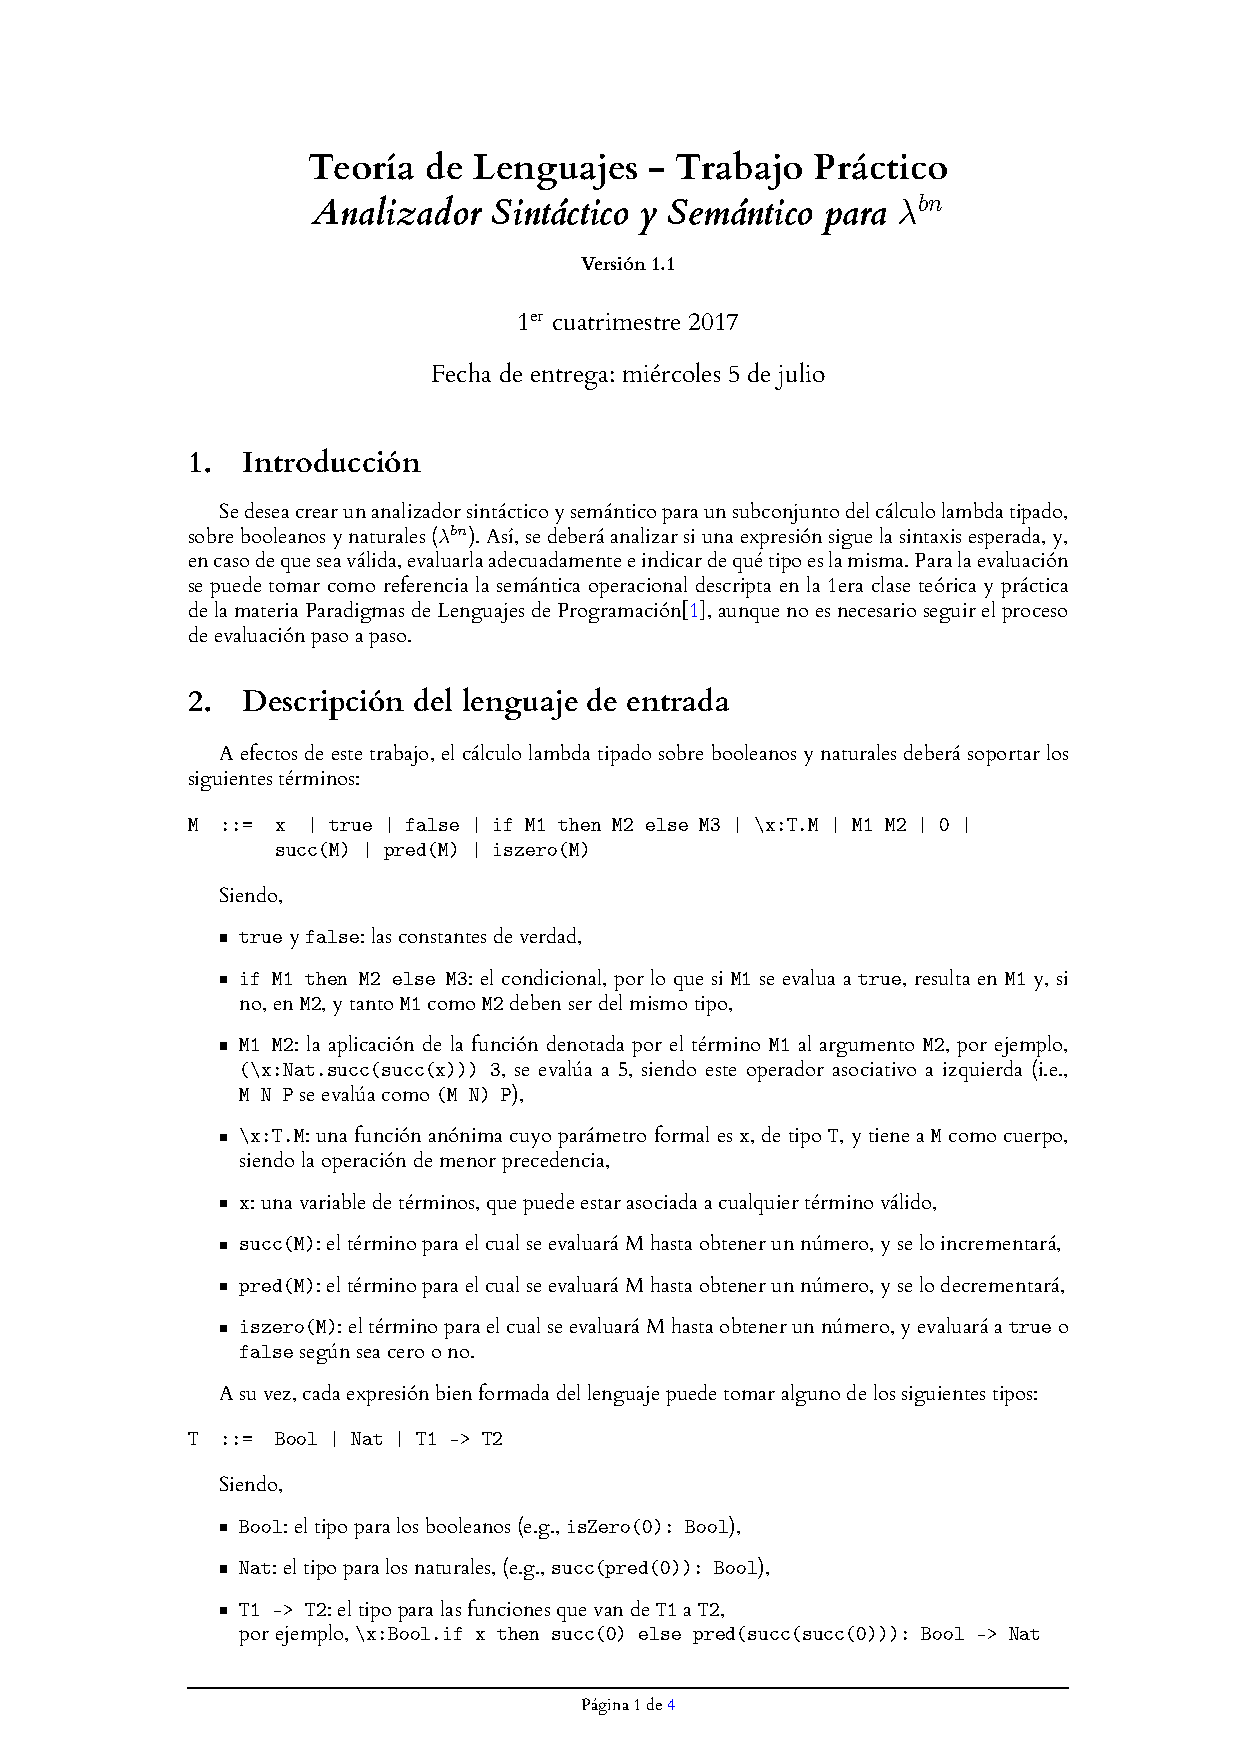
\includepdf[pages={1},pagecommand=\section{Enunciado},offset=40 -75]{enunciado.pdf}
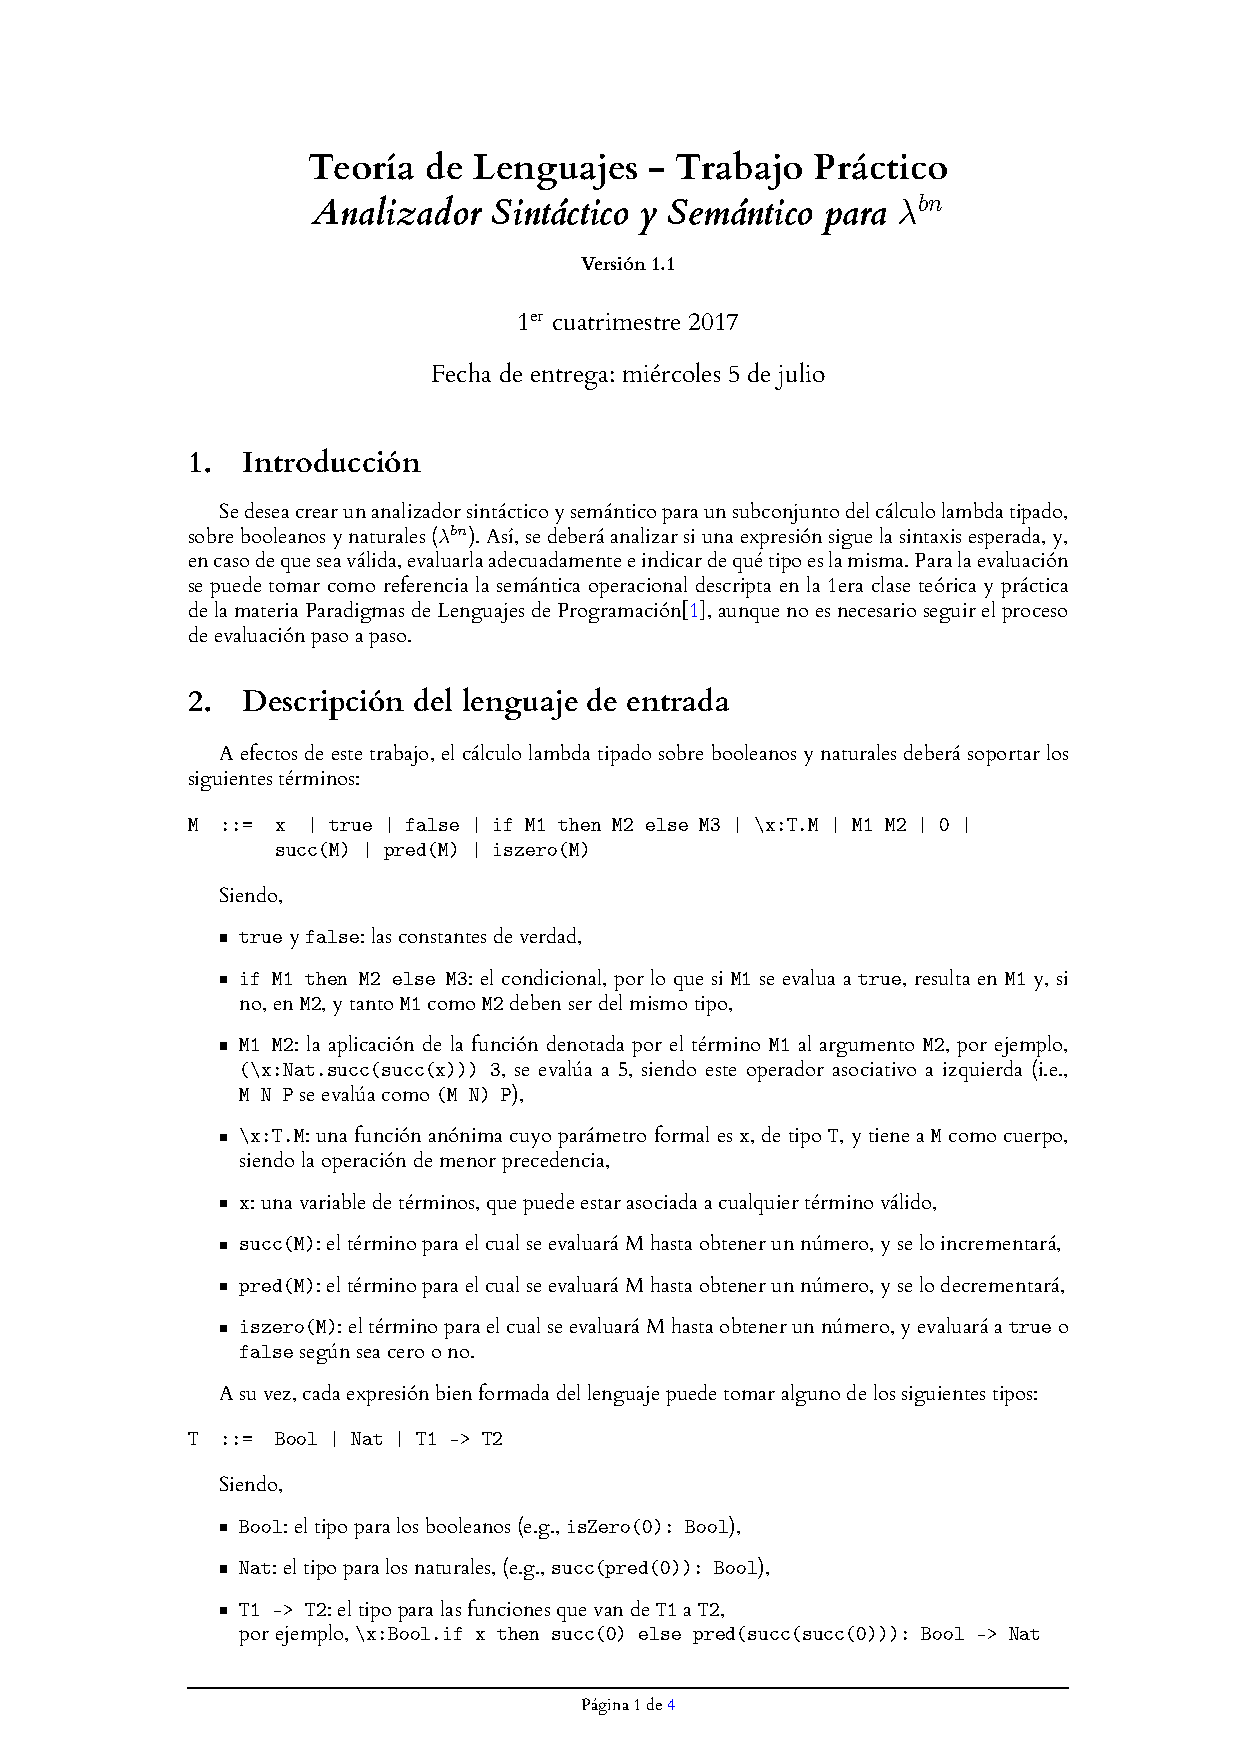
\includepdf[pages={1,2,3,4},offset=40 -75]{enunciado.pdf}

\end{document}
